\documentclass[9pt]{revtex4-1}
\usepackage{graphicx}
\title{Lista de galaxias candidatas -- DR1}

\begin{document}
\maketitle

\section{DR1}
\subsection{Candidatas seguras}


\begin{center}
\begin{tabular}{ l c c }
Nombre & Tipo & Redshift (z) \\
\hline
\hline \\
UGC00312 & G & 0.014507 -- 0.014557 \\
UGC07012 & G & 0.010277 \\
UGC08733 & G & 0.007799 \\
UGC09476 & Ggroup -- G & 0.010881 \\
\end{tabular}
\end{center}

\begin{figure}[h!]
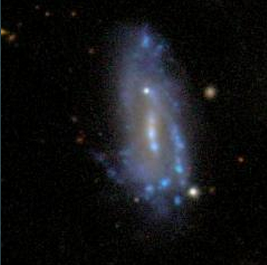
\includegraphics[scale=0.3]{UGC00312.png}
\caption{UGC00312}
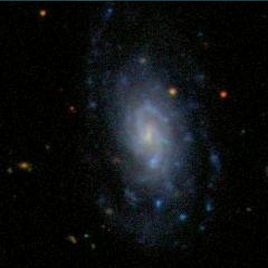
\includegraphics[scale=0.3]{UGC07012.png}
\caption{UGC07012}
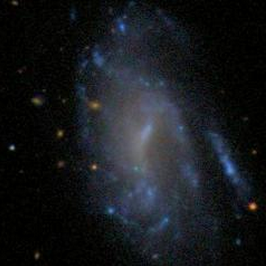
\includegraphics[scale=0.3]{UGC08733.png}
\caption{UGC08733}
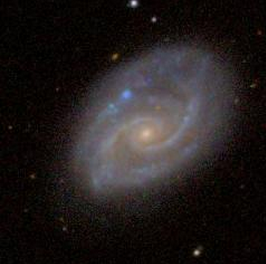
\includegraphics[scale=0.3]{UGC09476.png}
\caption{UGC09476}
\end{figure}

%\section{Probablemente candidatas}

\begin{center}
\begin{tabular}{ l c c }
Nombre & Tipo & Redshift (z) \\
\hline
\hline \\
NGC7819 & G -- Ggroup & 0.016538 -- 0.017299 \\
NGC0477 & G (creo que se vi\'o una supernova -- SN2002jy) & 0.019600 \\
NGC2916 & G *(Revisar con Jaime) & *Revisar con Jaime \\
NGC7321 & G (dos SN (2013di, 2008gj)) & 0.023833 \\
IC1256  & G & 0.015778 \\

\end{tabular}
\end{center}

\begin{figure}[h]
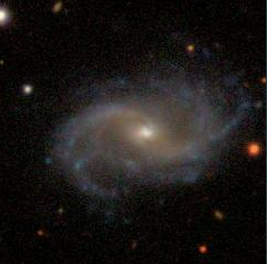
\includegraphics[scale=0.3]{NGC7819.png}
\caption{NGC7819}
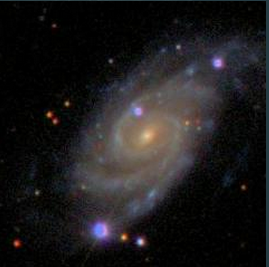
\includegraphics[scale=0.3]{NGC0477.png}
\caption{NGC0477}
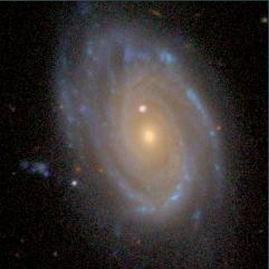
\includegraphics[scale=0.3]{NGC2916.png}
\caption{NGC2916}
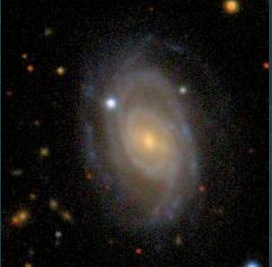
\includegraphics[scale=0.3]{NGC7321.png}
\caption{NGC7321}
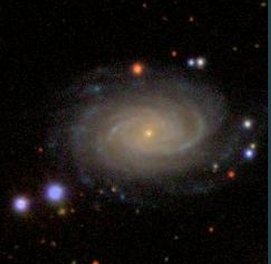
\includegraphics[scale=0.3]{IC1256.png}
\caption{IC1256}
\end{figure}

%\section{Revisar}

\begin{center}
\begin{tabular}{ l c c }
Nombre & Tipo & Redshift (z) \\
\hline
\hline \\
NGC0036 & G & 0.020114 \\
NGC0776 & G (SN1999di) & 0.016415 \\
NGC4210 & G (SN2002ho) & 0.009113 \\
NGC4185 & G (SN1982C)  & 0.013022 \\
IC0776  & G & 0.008232 \\
NGC5000 & G (SN2003el) & 0.018706 \\
UGC08781 & G & 0.025324 \\
NGC5406 & G (SN1977B) & 0.017352

\end{tabular}
\end{center}

\begin{figure}[h]
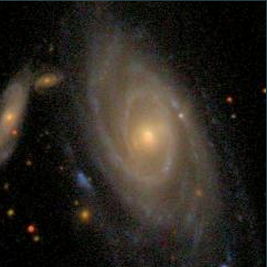
\includegraphics[scale=0.3]{NGC0036.png}
\caption{NGC0036}
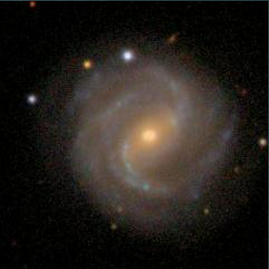
\includegraphics[scale=0.3]{NGC0776.png}
\caption{NGC0776}
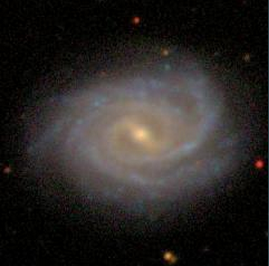
\includegraphics[scale=0.3]{NGC4210.png}
\caption{NGC4210}
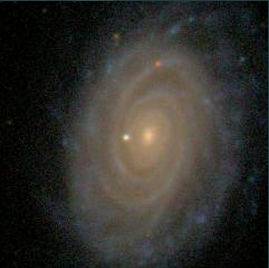
\includegraphics[scale=0.3]{NGC4185.png}
\caption{NGC4185}

\end{figure}

\begin{figure}[h]
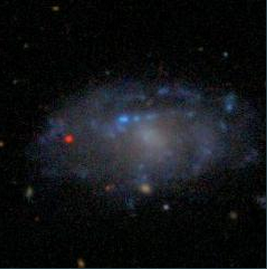
\includegraphics[scale=0.3]{IC0776.png}
\caption{IC0776}
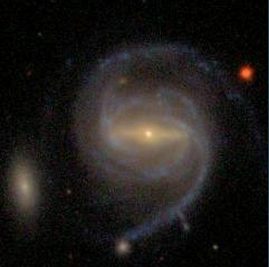
\includegraphics[scale=0.3]{NGC5000.png}
\caption{NGC5000}
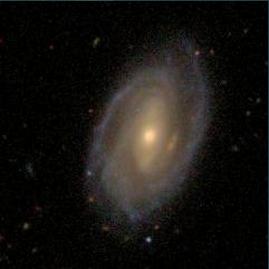
\includegraphics[scale=0.3]{UGC08781.png}
\caption{UGC08781}
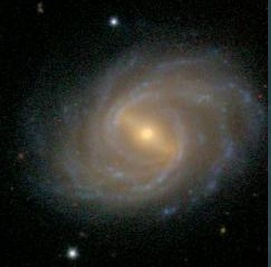
\includegraphics[scale=0.3]{NGC5406.png}
\caption{NGC5406}
\end{figure}

\section{DR2}

\begin{center}

\begin{tabular}{ l c c }

Nombre & G & Redshift (z) \\
\hline
\hline \\
UGC09476 & Ggroup -- G & 0.010881 \\
NGC5888  & G (SN2010fv, 2007Q) & 0.029123 \\
NGC6004  & G & 0.012762 \\
IC4566   & G & 0.019260 \\
NGC6063  & G (SN1999ac) & 0.009500 \\
NGC6154  & G & 0.020064 \\
IC1256   & G & 0.015778 \\
NGC6941  & G & 0.020761 \\
UGC11649 & G & UGC11649 \\

\end{tabular}

\end{center}

\end{document}